\documentclass{beamer}
  \usepackage[utf8]{inputenc}
  \usepackage{graphicx}
  \usepackage{array}
  \usepackage{url}
  \usepackage{ amssymb }
  \usepackage{amsmath}
  \usepackage{tikz}
  \usetikzlibrary{arrows,automata}
  \usetheme{Warsaw}

  \title{Bertrand competition in networks}
  \author{Benjamin Fasquelle, Arthur Queffelec, Raphaël Truffet}
  \institute{École Normale Supérieure de Rennes, département Informatique et Télécommunications}

  \begin{document}

\setbeamercolor{structure}{fg=magenta}

\AtBeginSection[]
{
  \begin{frame}<beamer>
    \frametitle{Sommaire}
{\scriptsize\tableofcontents[currentsection]
}
  \end{frame}
}

\addtobeamertemplate{footline}{\hfill\insertframenumber/\inserttotalframenumber}

  \begin{frame}
  \titlepage
  \end{frame}


\begin{frame}
  \tableofcontents
  \end{frame}


\section{Introduction and motivations}

\begin{frame}
Internet: effectiveness of its current routing protocols in finding good routes and ensuring quality
of service. 

\begin{alertblock}{Problems}
Distributed growth and selfish use of resources
\end{alertblock}

\vspace{5mm}

A first solution: Congestion and Quality of Service based pricing

\vspace{5mm}

Unfortunately, the effectiveness of such approaches relies on the cooperation of the owners of resources on the Internet, or the ISPs.
But their primary objective is \textbf{to maximize their own market share and profit}.
\end{frame}



\begin{frame}
Given a large combinatorial
market such as the Internet, suppose that:
\begin{itemize}
\item the owners of resources selfishly price
their product so as to maximize their profit
\item consumers selfishly purchase
bundles of products to maximize their utility
\end{itemize}

\begin{alertblock}{}
How does this effect the functioning
of the market as a whole?
\end{alertblock}
\end{frame}


\begin{frame}{State of the art}
Economists have traditionally studied the properties of equilibria that emerge
in pricing games with competing firms in \textbf{single-item markets}.

\begin{itemize}
\item two or a few competing firms lead to a socially-optimal
equilibrium
\item a monopoly can cause an inefficient allocation
by selfishly maximizing its own profit (bounded by a logarithmic factor in the disparity between
consumer values, as well as by a logarithmic factor in the number of consumers)
\end{itemize}

Those models ignore the combinatorial aspects of network pricing.
%namely that consumers have different geographic sources and destinations for their traffic, and goods (i.e., edges) are not pure substitutes, but rather
%are a complex mix of substitutes and complements, as defined by the network topology.
\end{frame}


\begin{frame}
Which properties of standard price equilbrium models carry over to network/combinatorial settings?
\begin{itemize}
\item Are equilibria still guaranteed to exist? 
\item Are equilibria fully efficient?
\item Does the answer depend in an interesting way on the network/demand structure?
\end{itemize}

We investigate these questions in general single-source single-sink networks (it captures the classical single-item setting), as well as multiple-source single-sink networks.
\end{frame}



\section{Network Pricing Game and Bertrand Competition}

\subsection{Network Pricing Game model}

\begin{frame}
A network pricing game (NPG) is characterized by a directed graph $G = (V, E)$
with edge capacities ${c_e}, e \in E$ , and a set of users (traffic matrix) endowed with
values.

Each edge is owned by a distinct ISP.
%The value associated with each chunk of traffic represents the per-unit monetary value that the owner of that chunk obtains upon sending this traffic from its source to its destination.
User values are represented in the form of demand curves, $D_{(s,t)}$ ,
for every source-destination pair $(s, t)$, where for every $\ell$, $D_{(s,t)} (\ell)$ represents the
amount of traffic with value at least $\ell$.
\end{frame}

\begin{frame}
%When the network has a single source-sink pair, we drop the subscript (s, t). 
We use D to denote the “demand suite”, or the collection of these demand curves, one for each source-sink pair.
Without loss of generality, the minimum value is $1$, that is, $D_{(s,t)} (1) = F^{tot}_{s,t}$ for all pairs $(s, t)$,
and we use $\mathcal{L}$ to denote the maximum value:
\begin{center}
$\mathcal{L} = sup\{\ell|D_{(s,t)} (\ell) > 0\}$
\end{center}
\end{frame}



\subsection{Prices of anarchy and stability}

\begin{frame}
We evaluate the Nash equilibria of these games with respect to two objectives (social value and profit).

\begin{itemize}
\item $\textbf{Val}(S)$: social value of a state $S$ of the network
\item $\textbf{Pro}(S)$: total utility of all the ISPs, or the total payment made by all users.
\end{itemize}

%The social value of a state $S$ of the network, , is defined to be the total utility of all the agents in the system.
% specifically, the total value obtained by all the users, minus the prices paid by the users, plus the profits (prices) earned by all the ISPs. Since prices are endogenous to the game, this is equivalent to the total value obtained by all the users, and we will use this latter expression to evaluate it throughout the paper.

%The worst such value over all Nash equilibria is captured by the price of anarchy:
%the price of anarchy of the NPG with respect to social value, POA Val , is defined to be the minimum over all Nash equilibria S in N of the ratio of the social value of the equilibrium to the optimal achievable value Val  :
\begin{block}{Price of Anarchy}
\begin{center}
$POA_{Val} (G, D) = \frac{min_{S \in N (G,D)} Val(S)}{Val *}$

$POA_{Pro} (G, D) = \frac{min_{S \in N (G,D)} Pro(S)}{Pro *}$
\end{center}
\end{block}

%Here, Val  is the maximum total value achievable while satisfying all the capacity constraints in the network (this can be computed by a simple flow LP). Likewise, POA Pro denotes the price of anarchy with respect to profit:

%Here Pro(S) is the total utility of all the ISPs, or the total payment made by all users. The optimal profit Pro  is defined to be the maximum profit over all states in which users are at equilibrium, and capacity constraints are satisfied.


%In instances with a large price of anarchy, we also study the performance of the best Nash equilibria and provide lower bounds for it. The price of stability of a game is defined to be the maximum over all Nash equilbria in the game of the ratio of the value of the equilibrium to the optimal achievable value. We use POS Val and POS Pro to denote the price of stability with respect to social value and profit respectively.

\begin{block}{Price of Stability}
\begin{center}
$POS_{Val} (G, D) = \frac{max_{S \in N (G,D)} Val(S)}{Val *}$

$POS_{Pro} (G, D) = \frac{max_{S \in N (G,D)} Pro(S)}{Pro *}$
\end{center}
\end{block}
\end{frame}




\subsection{Classic Bertrand Competition}

\begin{frame}{Classic Bertrand Competition}

\end{frame}


\subsection{B.C. in NPG}

\begin{frame}
We extend the classic Bertrand model of competition to network pricing. The
NPG has two stages.

In the first stage, each ISP (edge) e picks a price n e .

In the second stage each user picks paths between its source and destination to send
its traffic. We assume that users can split their traffic into infinitesimally small
chunks, and spread it across multiple paths, or send fractional
P amounts of traffic.
Each user picks paths to maximize her utility, u = v - min P e in P e , where the
minimum is over all paths P from the user’s source to its destination, and v is
its value (or sends no flow if the minimum total price is larger than its value v).
This selection of paths determines the amount of traffic f e on each edge.

ISP e’s
utility is given by f e e if f e  c e , and  otherwise. ISPs are selfish and set
prices to maximize their utility.
\end{frame}


\section{Nash Equilibrium}

\subsection{NPG in single commodity}

\begin{frame}{NPG in single commodity}
  %Every customer has the same source and sink.
  The equilibrium of the NPG depends on the presence of competition in the network and the ammount of monopolies.
  \begin{definition}[Monopoly]
    An edge is monopolized over a user if its removal causes the non-reachability of the destination.
  \end{definition}
\end{frame}

\begin{frame}{Absence of monopoly}
  Without monopolies from any providers, the competition will decrease the prices to obtain a good social value. If a provider wishes to increase the price of an edge, he will be punish by the lack of users.
  \begin{theorem}
    In a single commodity network with no monopolies, \(POA_{Val} = 1\).% Furthermore, there exist instances with \(POS_{Pro} = \theta(\mathcal{L})\)
  \end{theorem}
  \center
  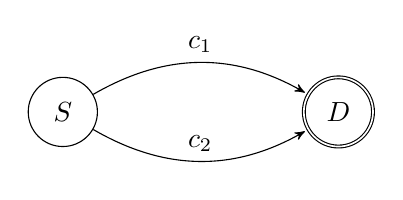
\begin{tikzpicture}[->,>=stealth',shorten >=1pt,auto,node distance=3.5cm,
      scale = 1,transform shape]

    \node[state] (S) {$S$};
    \node[state,accepting] (D) [right of=S] {$D$};

    \path (S) edge [bend left] node {$c_1$} (D)
    (S) edge [bend right] node {$c_2$} (D);

    \end{tikzpicture}
\end{frame}

\begin{frame}{Single monopoly}
  \begin{theorem}
    In a single commodity network with a single monopoly. \(POA_{Pro} = 1\) and \(POA_{Val} = O(log \mathcal{L})\).
    %Moreover, there exist instances with \(POS_{Val} = \theta(log \mathcal{L})\).
  \end{theorem}
  \center
  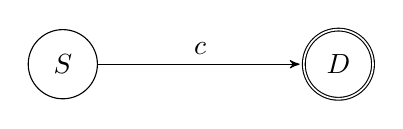
\begin{tikzpicture}[->,>=stealth',shorten >=1pt,auto,node distance=3.5cm,
      scale = 1,transform shape]

    \node[state] (S) {$S$};
    \node[state,accepting] (D) [right of=S] {$D$};

    \path (S) edge node {$c$} (D);

    \end{tikzpicture}
\end{frame}

\begin{frame}{Multiple monopolies}
  %\begin{theorem}
  %  For every B, there exists a single-source single-sink instance of the NPG containing 2 monopolies, with \(\mathcal{L} = 2\), and \(POA_{Val}\), \(POA_{Pro} = \Omega(B)\).
  %\end{theorem}
  \begin{theorem}
    In all single-commodity graphs with \(k > 1\) monopolies, \(POS_{Val}\), \(POS_{Pro} = O(\mathcal{L}^{k-1})\).% There exists a family of single-commodity instances with \(POS_{Val}\), \(POS_{Pro} = \Omega(\mathcal{L}^{k-1})\), where \(k\) is the number of monopolies.
  \end{theorem}
  \center
  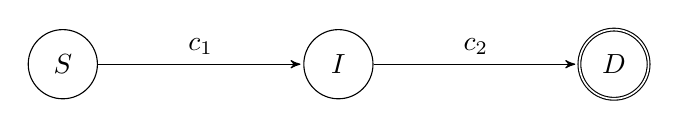
\begin{tikzpicture}[->,>=stealth',shorten >=1pt,auto,node distance=3.5cm,
      scale = 1,transform shape]

    \node[state] (S) {$S$};
    \node[state] (I) [right of=S]  {$I$};
    \node[state,accepting] (D) [right of=I] {$D$};

    \path (S) edge node {$c_1$} (I)
    (I) edge node {$c_2$} (D);

    \end{tikzpicture}
\end{frame}


\subsection{NPG ( n source / 1 sink)}


\begin{frame}
Next we study the NPG in graphs with more general traffic matrix. Specifically
different users have different sources, but a common sink. We assume that the
network is a DAG with a single sink, and focus on instances that contain no
monopolies 5 . Theorem 1 already shows that the price of stability with respect
to profit can be quite large in this case. The main question we address here
is whether competition drives down prices and enables a near socially optimal
equilibrium just as in the single-commodity case.
The results are surprisingly pessimistic. We find that there are networks with
no pure equilibria.
\end{frame}


\begin{frame}
Theorem 5. There exists a multi-source single-sink instance of the NPG with
no monopolies that does not admit any pure Nash equilibria.
In networks that admit pure equilibria, the price of stability for social value can
be polynomial in L. This can happen (Theorem 6 below) even when the network
in question satisfies a certain strong-competition condition, specifically, (1) there
is sufficient path-choice - from every node in the graph, there are at least two
edge-disjoint paths to the sink, and (2) no edge dominates over a specific user in
terms of the capacity available to that user – removing any single edge reduces
the amount of traffic that any user or group of users can route by only a constant
fraction. We therefore attempt to isolate conditions that lead to a high price of
stability, and find two culprits:
1. Variations in demand curves across users-a very high value low traffic user
can pre-empt a low value high traffic user.
2. Congestion in the network—congestion in one part of the network (owing to
low capacity), can get “carried over” to a different part of the network (in
the form of high prices) due to the ISPs’ selfishness.
Each condition alone can cause the network to have a high price of stability.
Theorem 6. There exists a family of multiple-source single-sink instances sat-
isfying strong competition and containing uniform demand such that POS Val =
omega(poly L, poly N ), where N is the size of the network. There exists a family
of multiple-source single-sink instances satisfying strong competition and with
sparsity 1 such that POS Val = omega(poly L, poly N ).
Here uniformity of demand and sparsity defined as follows.
Definition 2. An instance of the NPG, (G, D), with multiple commodities and
a single sink t is said to contain uniform demand if there exists a demand curve
D such that for all s, D (s,t) is either zero, or equal to a scalar F s,t times D.
Definition 3. Given a capacitated graph and a demand matrix, the sparsity of
a cut in the graph with respect to the demand is the ratio of the total capacity
of the cut to the total demand between all pairs (s, t) separated by the cut. The
sparsity of the graph is the minimum of these sparsities over all cuts in the graph.
\end{frame}


\begin{frame}
Fortunately, in the absence of the two conditions above, the network behaves
well. In particular, we consider a certain class of DAGs called traffic-spreaders
in which equilibria are guaranteed to exist, and show that when demand is
uniform, the price of stability with respect to the social value is at most 1/alpha,
where alpha is the sparsity of the network. We conjecture that this bound on the
price of stability holds for all DAGs that admit pure equilibria.
Definition 4. A DAG with sink t is said to be a traffic spreader if for every
node v in the graph, and every two distinct paths P 1 and P 2 from v to t, any
maximal common subpath of P 1 and P 2 is a prefix of both the paths.
Theorem 7. Let (G, D) be a uniform-demand instance of the NPG where G
is a traffic spreader and contains no monopolies, and all sources in the graph
are leaves, that is, their in-degree is 0. Then (G, D) always admits a pure Nash
equilibrium, and POS Val inf= 1/alpha, where alpha is the sparsity of G with respect to D.We remark that for Theorem 7, we do not require the instance to satisfy strong
competition. This indicates that the amount of competition in the network has
lesser influence on its performance compared to its traffic distribution.
\end{frame}

\section{Conclusion}

\begin{frame}{Results}
\end{frame}

\begin{frame}{Strengths and weaknesses}
We consider a simplistic model for network pricing. A more realistic model should
take into account quality of service requirements of the users, which may be
manifested in the form of different values for different paths between the same
source-destination pairs. In general combinatorial markets it would also be in-
teresting to consider the effect of production costs on the pricing game, andthis may change the behavior of the market considerably. Finally, an alternate
model of competition in two-sided markets is for the sellers to commit to produc-
ing certain quantities of their product, and allowing market forces to determine
the demand and prices. This two-stage game, known as “Cournot competition”,
may lead to better or worse equilibria compared to Bertrand competition.
\end{frame}




\end{document}
